% 请确保文件编码为utf-8,使用XeLaTex进行编译,或者通过overleaf进行编译

\documentclass[answers]{exam}  % 使用此行带有作答模块
% \documentclass{exam} % 使用此行只显示题目

\usepackage{xeCJK}
\usepackage{zhnumber}
\usepackage{graphicx}
\usepackage{hyperref}
\usepackage{amsmath}
\usepackage{booktabs}
\usepackage{enumerate}

\pagestyle{headandfoot}
\firstpageheadrule
\firstpageheader{南京大学}{数字信号处理}{习题集二}
\runningheader{南京大学}
{数字信号处理}
{习题集二}
\runningheadrule
\firstpagefooter{}{第\thepage\ 页(共\numpages 页)}{}
\runningfooter{}{第\thepage\ 页(共\numpages 页)}{}

% no box for solutions
% \unframedsolutions

\setlength\linefillheight{.5in}

% \renewcommand{\solutiontitle}{\noindent\textbf{答:}}
\renewcommand{\solutiontitle}{\noindent\textbf{解:}\par\noindent}

\renewcommand{\thequestion}{\zhnum{question}}
\renewcommand{\questionlabel}{\thequestion .}
\renewcommand{\thepartno}{\arabic{partno}}
\renewcommand{\partlabel}{\thepartno .}

\begin{document}
\Large

\centering{姓名:周韧哲 \qquad 学号:181220076 \qquad 邮箱:zhourz@smail.nju.edu.cn}

\begin{questions}
	
\question 已知周期信号$x(t)$的傅里叶级数表示式为$x(t) = 2 + 3\cos(2t) + 4\sin(2t) + 2\sin(3t + 30^{\circ}) - \cos(7t + 150^{\circ})$:

\begin{enumerate}[(1)]
	\item 求周期信号$x(t)$的基波角频率;
	\item 画出周期信号$x(t)$的幅度谱和相位谱。
\end{enumerate}

\begin{solution}
	\begin{enumerate}[(1)]
		\item $x(t)=2+x_1(t)+x_2(t)+x_3(t)+x_4(t)$,$T_1=T_2=\pi,T_3=\frac{2\pi}{3},T_4=\frac{2\pi}{7}$,因此$T=2T_1=2T_2=3T_3=7T_4=2\pi$,因此基波角频率为$w_1=\frac{2\pi}{T}=1$。
		\item $x(t)=2+5\cos(2t-53^{\circ})+2\cos(3t-60^{\circ})+\cos(7t+60^{\circ})$,所以其幅度谱和相位谱如图\ref{fig:1}图\ref{fig:2}:
	\end{enumerate}
\end{solution}
\begin{figure}
	\centering
	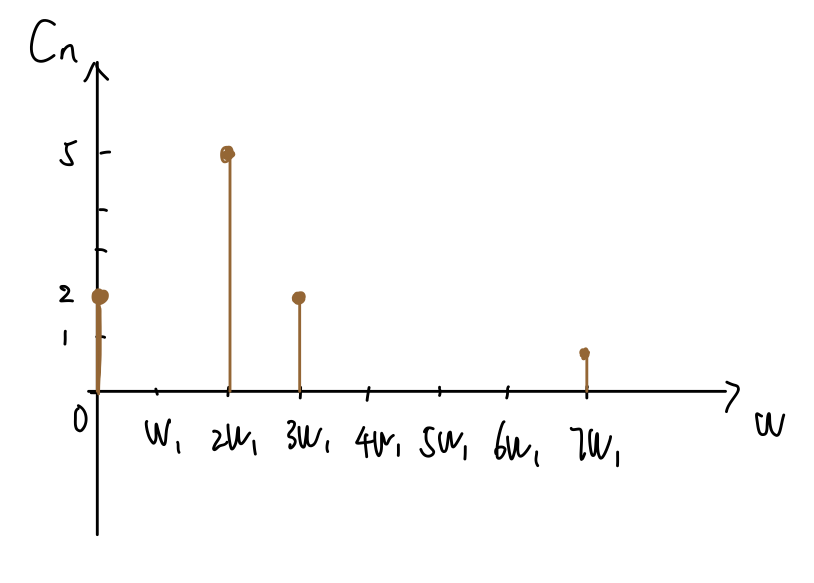
\includegraphics[width=0.5\textwidth]{pics/1-1.png}
	\caption{1-幅度谱}
	\label{fig:1}
\end{figure}
\begin{figure}
	\centering
	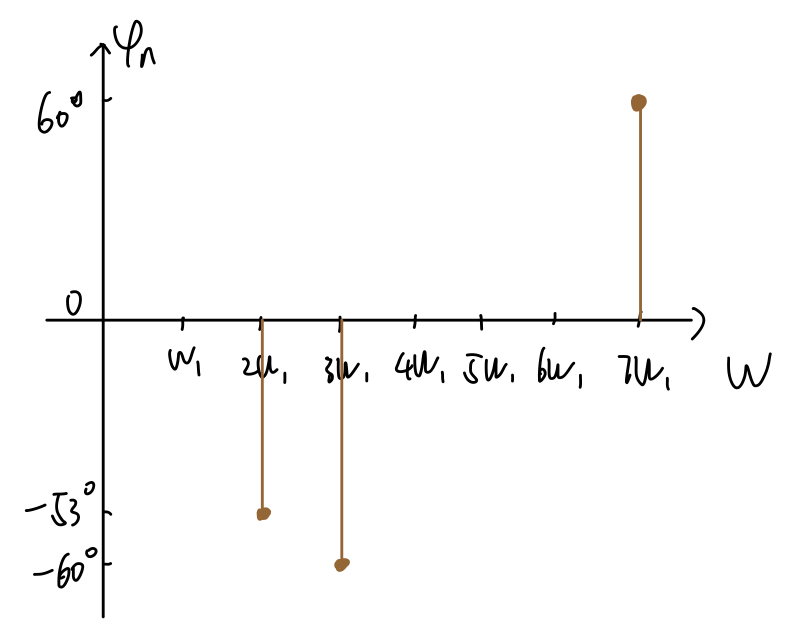
\includegraphics[width=0.5\textwidth]{pics/1-2.png}
	\caption{1-相位谱}
	\label{fig:2}
\end{figure}
\question 已知信号
\begin{equation}
	\nonumber
	x(t) = 
	\begin{cases}
		1 + \cos(t), \qquad |t| \leq \pi \\
		0, \qquad |t| > \pi
	\end{cases}	
\end{equation}
求该信号的傅里叶变换。

\begin{solution}
    \begin{align*}
    	X(jw)&=\int_{-\infty}^{\infty} x(t)e^{-jwt} dt\\ 
    	     &=\int_{-\pi}^{\pi} (1+\cos(t))(\cos(wt)-j\sin(wt)) dt\\
    	     &=\int_{-\pi}^{\pi} (1+\cos(t))\cos(wt)dt- \int_{-\pi}^{\pi} j(1+\cos(t))\sin(wt) dt\\
    	     &=\int_{-\pi}^{\pi} (1+\cos(t))\cos(wt)dt-0\\
    	     &=\int_{-\pi}^{\pi} \cos(wt)+\frac{1}{2}\cos((1-w)t)+\frac{1}{2}\cos((1+w)t)dt\\
    	     &=\frac{2\sin(w\pi)}{w}+\frac{\sin((1-w)\pi)}{1-w}+\frac{\sin((1+w)\pi)}{1+w}\\
    	     &=2\pi Sa(w\pi)+\pi Sa((1-w)\pi)+\pi Sa((1+w)\pi)
    \end{align*}
\end{solution}


\question 已知$x_1(t)$和$x(t)$的波形图如图\ref{fig:3}所示,$x_1(t)$的傅里叶变换为$X_1(j\omega)=2T \cdot Sa(\omega T)$,试利用傅里叶变换的尺度变换、位移和线性性质求$x(t)$的傅里叶变换。

\begin{figure}
	\centering
	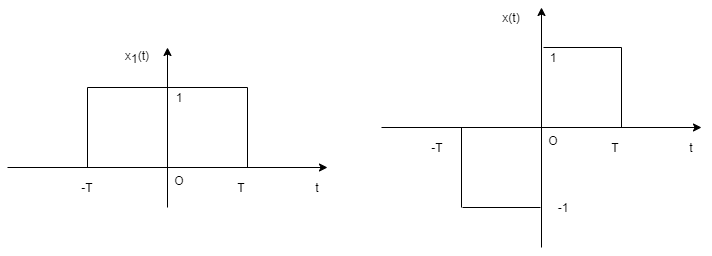
\includegraphics[width=\linewidth]{pics/dsp2-3.png}
	\caption{题目三图}
	\label{fig:3}
\end{figure}

\begin{solution}
	易知$x(t)=x_1(2t-T)-x_1(2t+T)$,所以
	\begin{align*}
		\mathcal{F}[x(t)]&=\mathcal{F}[x_1(2t-T)]-\mathcal{F}[x_1(2t+T)]\\
		&=\frac{1}{2}X_1(\frac{jw}{2})e^{-j\frac{wT}{2}}-\frac{1}{2}X_1(\frac{jw}{2})e^{j\frac{wT}{2}}\\
		&=\frac{1}{2}\times 2T\cdot Sa(\frac{wT}{2})e^{-j\frac{wT}{2}}-\frac{1}{2}\times 2T\cdot Sa(\frac{wT}{2})e^{j\frac{wT}{2}}\\
		&=T\cdot Sa(\frac{wT}{2})(e^{-j\frac{wT}{2}}-e^{j\frac{wT}{2}})
	\end{align*}
\end{solution}


\question 求图\ref{fig:4}所示对称周期矩形信号的傅里叶级数,三角形式和指数形式。

\begin{figure}
	\centering
	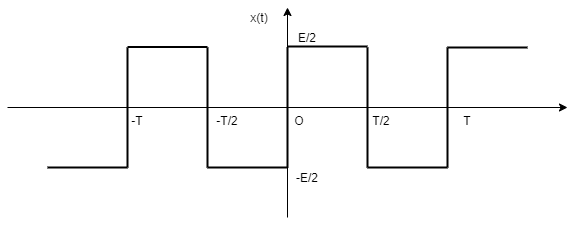
\includegraphics[width=\linewidth]{pics/dsp2-5.png}
	\caption{题目四图}
	\label{fig:4}
\end{figure}

\begin{solution}
	首先写出三角形式傅里叶级数:$$x(t)=a_0+\sum_{n=1}^{\infty}[a_n\cos(nw_1t)+b_n\sin(nw_1t)]$$其中$w_1=\frac{2\pi}{T}$。由于$x(t)$为奇信号且无直流分量,所以$a_0=0,a_n=0$。而
	\begin{align*}
		b_n&=\frac{2}{T}\int_{-\frac{T}{2}}^{\frac{T}{2}}x(t)\sin(nw_1t)dt\\
		&=\frac{4}{T}\int_{0}^{\frac{T}{2}}x(t)\sin(nw_1t)dt\\
		&=\frac{4}{T}\int_{0}^{\frac{T}{2}}\frac{E}{2}\sin(nw_1t)dt\\
		&=\frac{E}{n\pi}(1-\cos(n\pi))
	\end{align*}
    所以三角形式
    \begin{align*}
    	x(t)&=\sum_{n=1}^{\infty}\frac{E}{n\pi}(1-\cos(n\pi))\sin(nw_1t)\\
    	&=\sum_{n=1,3,\cdots}\frac{2E}{n\pi}\sin(\frac{2n\pi t}{T})
    \end{align*}
    指数形式为$$x(t)=\sum_{n=-\infty}^{\infty}X_ne^{jnw_1t}$$
    \begin{align*}
    	X_n&=\frac{1}{T}\int_{-\frac{T}{2}}^{\frac{T}{2}}x(t)e^{-jnw_1t}dt\\
    	   &=\frac{1}{T}[\int_{-\frac{T}{2}}^{0}x(t)e^{-jnw_1t}dt+\int_{0}^{
    	    \frac{T}{2}}x(t)e^{-jnw_1t}dt]\\
           &=\frac{1}{T}[\int_{-\frac{T}{2}}^{0}\frac{-E}{2}e^{-jnw_1t}dt+\int_{0}^{
           	\frac{T}{2}}\frac{E}{2}e^{-jnw_1t}dt]\\
           &=\frac{1}{T}[\frac{E}{2jnw_1}(1-e^{jn\pi})-\frac{E}{2jnw_1}(e^{-jn\pi}-1)]\\
           &=\frac{E}{4jn\pi}(2-e^{jn\pi}-e^{-jn\pi})\\
           &=\frac{E}{2jn\pi}(1-\frac{e^{jn\pi}+e^{-jn\pi}}{2})\\
           &=\frac{E}{2jn\pi}(1-\cos(n\pi))=\begin{cases}
           	\frac{E}{jn\pi} & \text{n is odd}\\
           	 0 & \text{n is even}
                       \end{cases}
    \end{align*}
    所以指数形式为$$x(t)=\sum_{n=\pm1,\pm3,\cdots}\frac{E}{jn\pi}e^{\frac{2n\pi t}{T}}$$
\end{solution}

\question 求图\ref{fig:5}所示周期锯齿信号的指数形式傅里叶级数,并大致画出频谱图。

\begin{figure}
	\centering
	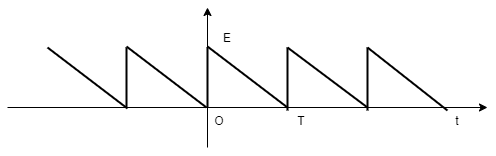
\includegraphics[width=\linewidth]{pics/dsp2-6.png}
	\caption{题目五图}
	\label{fig:5}
\end{figure}

\begin{solution}
	令$w_1=\frac{2\pi}{T}$,指数形式为$$x(t)=\sum_{n=-\infty}^{\infty}X_ne^{jnw_1t}$$
	\begin{align*}
		X_n&=\frac{1}{T}\int_{0}^{T}x(t)e^{-jnw_1t}dt\\
		&=\frac{1}{T}\int_{0}^{T}E(1-\frac{t}{T})e^{-jnw_1t}dt\\
		&=\frac{E}{T}[\int_{0}^{T}e^{-jnw_1t}dt-\frac{1}{T}\int_{0}^{T}te^{-jnw_1t}dt]
	\end{align*}
当$n=0$时,$X_0=\frac{E}{T}(T-\frac{T^2}{2T})=\frac{E}{2}$。当$n\neq0$时,上式的第一项积分为$\frac{e^{-j2n\pi}-1}{-jnw_1}=\frac{\cos(2n\pi)-j\sin(2n\pi)-1}{-jnw_1}=0$。而
\begin{align*}
	\frac{1}{T}\int_{0}^{T}te^{-jnw_1t}dt&=\int_{0}^{T}\frac{t}{-jnw_1T}de^{-jnw_1t}\\
	&=\frac{1}{-jnw_1T}(te^{-jnw_1t}\bigg|_0^T-\int_{0}^{T}e^{-jnw_1t}dt)\\
	&=\frac{e^{-j2n\pi}}{-jnw_1}
\end{align*}
因此$$X_n=\frac{E}{T}(0-\frac{e^{-j2n\pi}}{-jnw_1})=\frac{E}{j2n\pi}$$
因此指数形式为$$x(t)=\frac{E}{2}+\sum_{n\neq 0,n\in\mathbf{Z}}\frac{E}{j2n\pi}e^{jnw_1t}$$
其幅度谱和相位谱如图\ref{fig:11}图\ref{fig:12}所示。
\end{solution}
\begin{figure}
	\centering
	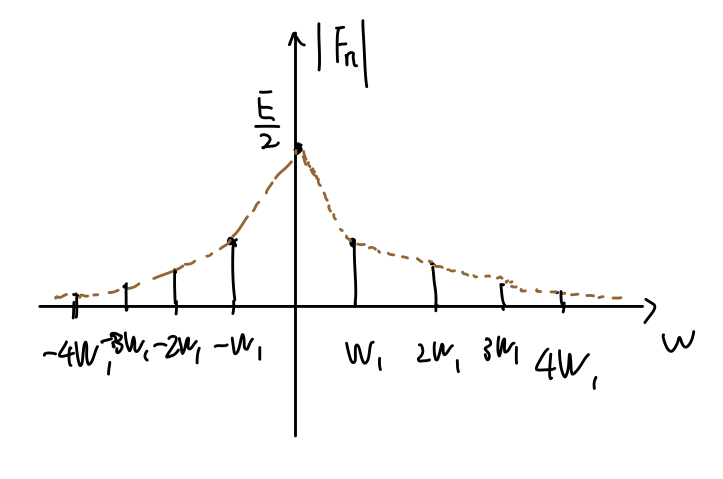
\includegraphics[width=0.5\textwidth]{pics/5-1.png}
	\caption{5-幅度谱}
	\label{fig:11}
\end{figure}
\begin{figure}
	\centering
	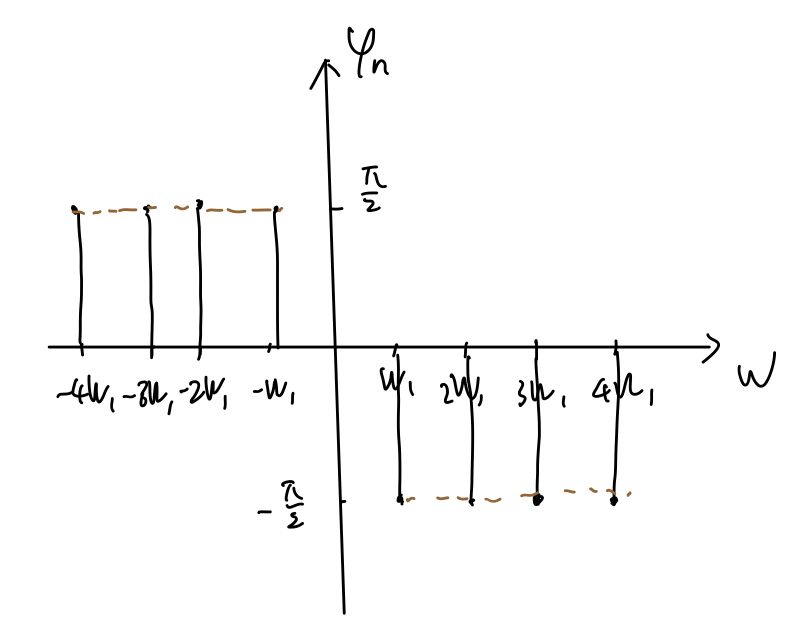
\includegraphics[width=0.5\textwidth]{pics/5-2.png}
	\caption{5-相位谱}
	\label{fig:12}
\end{figure}
\question 求图\ref{fig:6}所示锯齿脉冲与单周正弦脉冲的傅里叶变换。
\begin{figure}
	\centering
	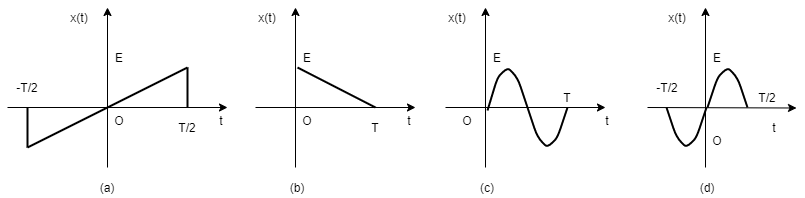
\includegraphics[width=\linewidth]{pics/dsp2-7.png}
	\caption{题目六图}
	\label{fig:6}
\end{figure}

\begin{solution}
	\begin{enumerate}[(a)]
		\item 当$w\neq0$时,\begin{align*}
			X(jw)&=\int_{-\frac{T}{2}}^{\frac{T}{2}}\frac{2Et}{T}e^{-jwt}dt\\
			&=\frac{2E}{-jwT}\int_{-\frac{T}{2}}^{\frac{T}{2}}tde^{-jwt}\\
			&=\frac{2E}{-jwT}(T\cos(\frac{wT}{2})-\frac{2}{w}\sin(\frac{wT}{2}))\\
			&=\frac{2E}{-jw}(\cos(\frac{wT}{2})-Sa(\frac{wT}{2}))
		\end{align*}而$x(t)$无直流分量,所以$X(0)=0$。
	    \item 当$w\neq0$时,\begin{align*}
	    	X(jw)&=\int_{0}^{T}(E-\frac{Et}{T})e^{-jwt}dt\\
	    	&=\int_{0}^{T}Ee^{-jwt}dt-\frac{E}{T}\int_{0}^{T}te^{-jwt}dt\\
            &=\frac{E}{w^2T}(1-e^{-jwT}-jwT)
	    \end{align*}当$w=0$时$X(0)=\int_{0}^{T}(E-\frac{Et}{T})dt=\frac{ET}{2}$。
        \item 令$w_1=\frac{2\pi}{T}$,则
             \begin{align*}
             	X(jw)&=\int_{0}^{T}E\sin(w_1t)e^{-jwt}dt\\
             	&=\frac{E}{2j}\int_{0}^{T}(e^{(w_1-w)}t-e^{-j(w_1+w)t})dt\\
             	&=\frac{Ew_1}{w_1^2-w^2}(1-e^{-jwT})
             \end{align*}当$w=w_1$时,$X(jw_1)=\frac{E}{2j}\int_{0}^{T}(1-e^{\frac{-j4\pi t}{T}})dt=\frac{ET}{2j}$
         \item 令$w_1=\frac{2\pi}{T}$,则
         \begin{align*}
         	X(jw)&=\int_{-\frac{T}{2}}^{\frac{T}{2}}E\sin(w_1t)e^{-jwt}dt\\
         	&=\frac{E}{2j}\int_{-\frac{T}{2}}^{\frac{T}{2}}(e^{(w_1-w)}t-e^{-j(w_1+w)t})dt\\
         	&=\frac{j2Ew_1}{w^2-w_1^2}\sin(\frac{wT}{2})
         \end{align*}当$w=w_1$时,$X(jw_1)=\frac{E}{2j}\int_{-\frac{T}{2}}^{\frac{T}{2}}(1-e^{\frac{-j4\pi t}{T}})dt=\frac{ET}{2j}$
	\end{enumerate}
\end{solution}


\question 分别求图\ref{fig:10}所示$X(j\omega)$的傅里叶逆变换。
\begin{figure}
	\centering
	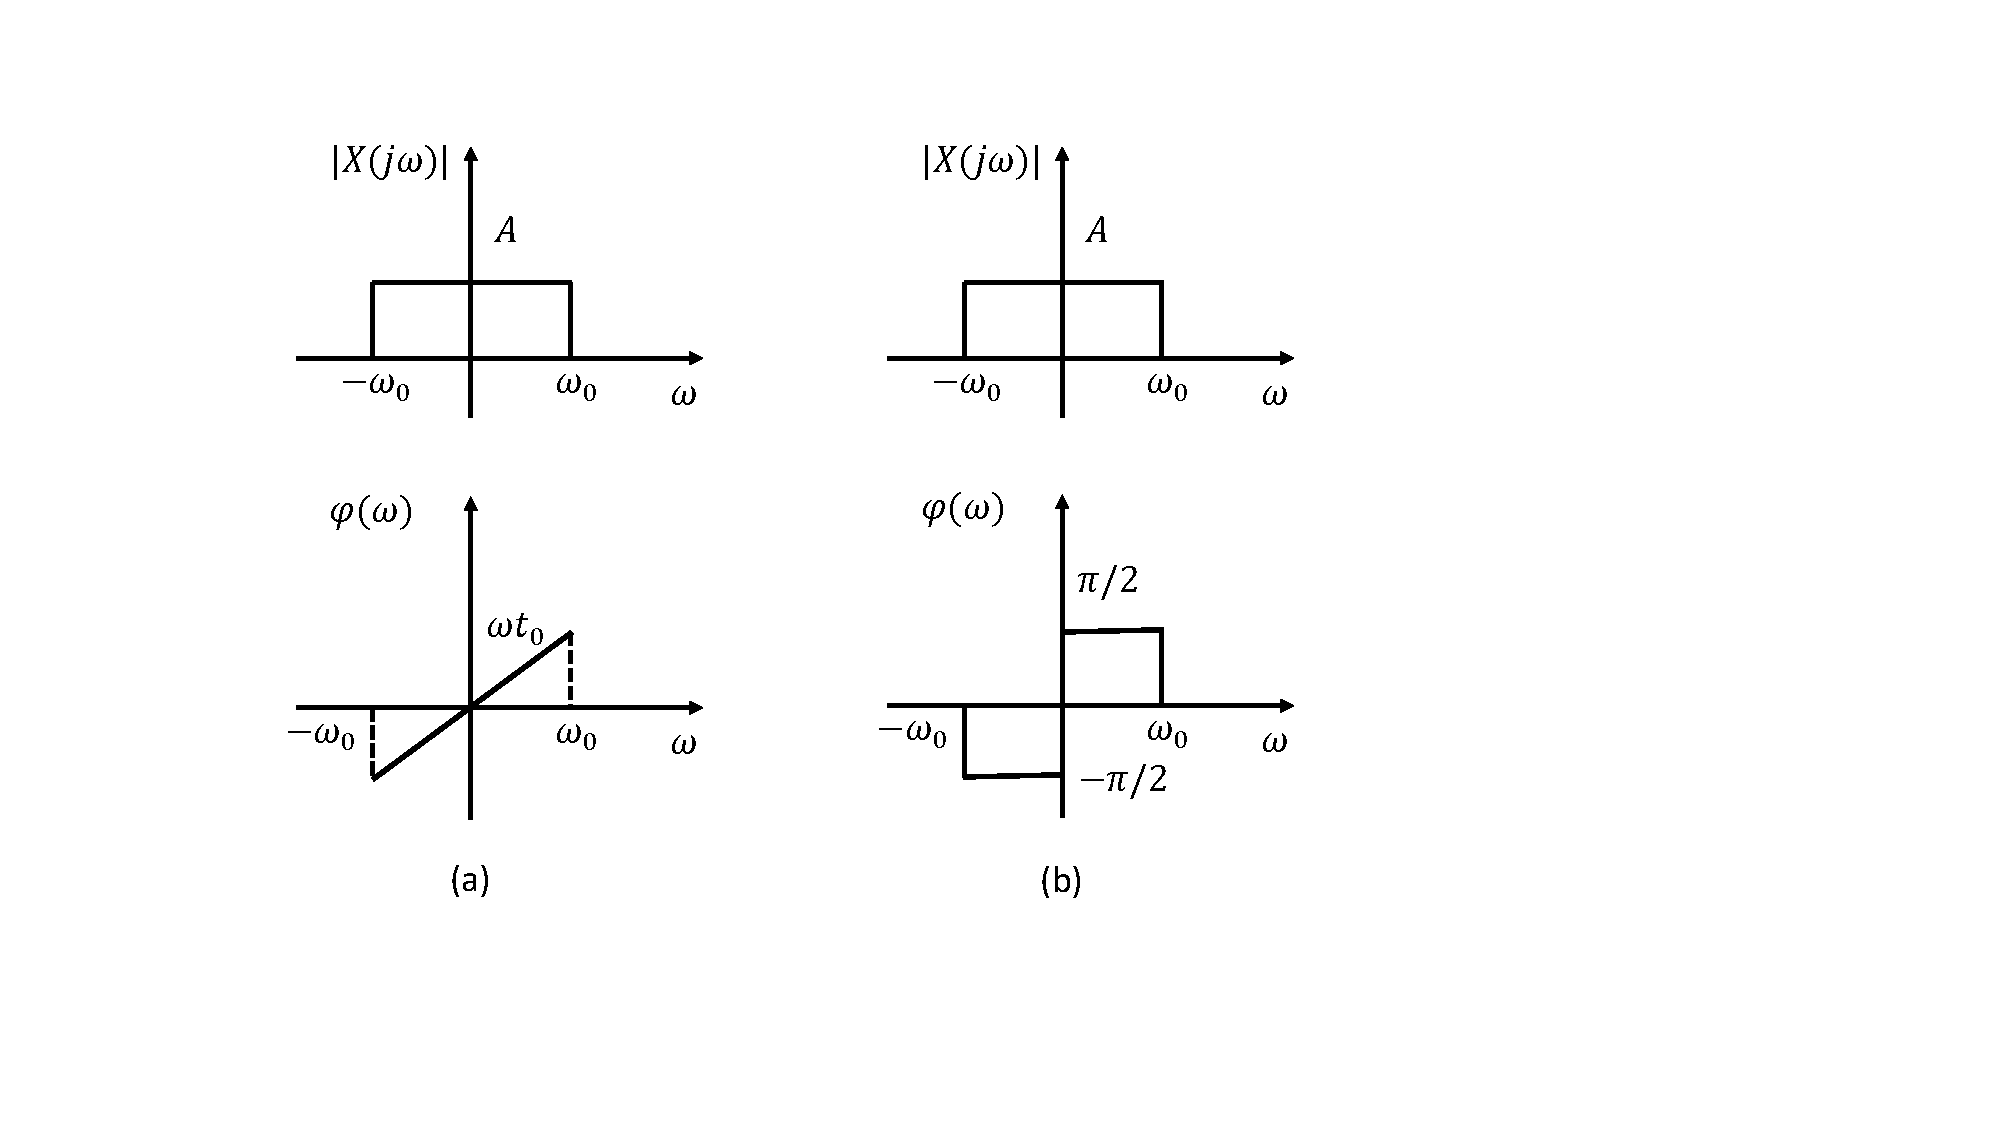
\includegraphics[width=\linewidth]{pics/dsp2-8.pdf}
	\caption{题目七图}
	\label{fig:10}
\end{figure}

\begin{solution}
	\begin{enumerate}[(a)]
		\item 易知$X(jw)=Ae^{jwt_0}$,所以\begin{align*}
			x(t)&=\frac{1}{2\pi}\int_{-w_0}^{w_0}Ae^{jwt_0}e^{jwt}dw\\
			&=\frac{A}{2\pi}\int_{-w_0}^{w_0}e^{j(t_0+t)w}dw\\
			&=\frac{A}{\pi(t+t_0)}\sin(w_0(t+t_0))\\
			&=\frac{Aw_0}{\pi}Sa(w_0(t+t_0))
		\end{align*}
	    \item 易知$X(jw)=Ae^{j\frac{\pi}{2}sgn(w)}$,其中$sgn(x)$为符号函数,所以\begin{align*}
	    	x(t)&=\frac{1}{2\pi}\int_{-w_0}^{w_0}Ae^{j\frac{\pi}{2}sgn(w)}e^{jwt}dw\\
	    	&=\frac{1}{2\pi}[\int_{-w_0}^{0}-jAe^{jwt}dw+\int_{0}^{w_0}jAe^{jwt}dw]\\
	    	&=\frac{A}{\pi t}[\frac{e^{-jw_0t}+e^{jw_0t}}{2}-1]\\
	    	&=\frac{A}{\pi t}(\cos(w_0t)-1)
	    	\end{align*}
	\end{enumerate}
\end{solution}


\question 利用微分定理求图\ref{fig:8}所示梯形脉冲的傅里叶变换,并大致画出$\tau=2\tau_1$情况下该脉冲的频谱图。
\begin{figure}
	\centering
	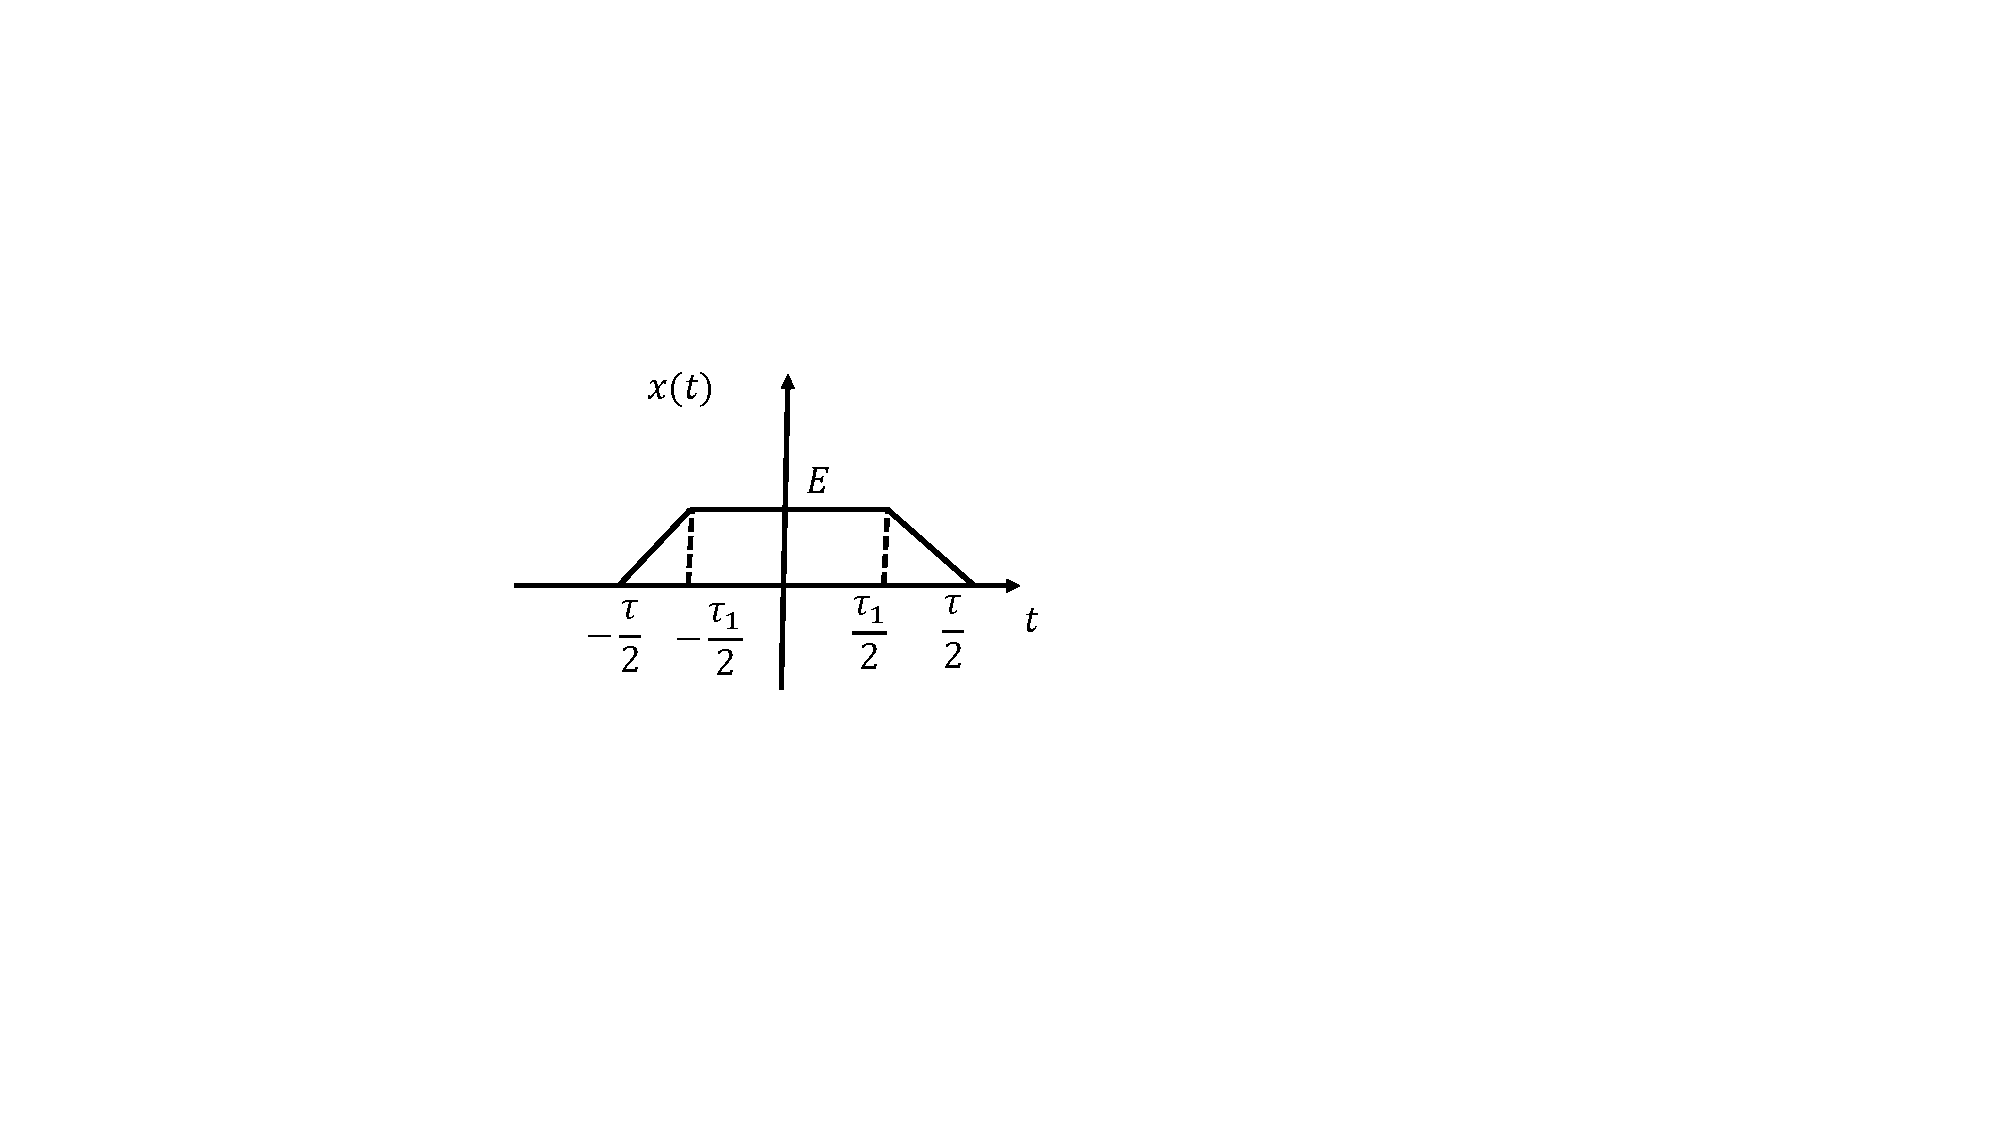
\includegraphics[width=\linewidth]{pics/dsp2-10.pdf}
	\caption{题目八图}
	\label{fig:8}
\end{figure}

\begin{solution}
	容易画出$x(t)$的一阶导数和二阶导数如图\ref{fig:13}。易得$\mathcal{F}[\frac{d^2x(t)}{dt^2}]=(jw)^2X(jw)$,而$$\frac{d^2x(t)}{dt^2}=\frac{2E}{\tau-\tau_1}[\delta(t+\frac{\tau}{2})-\delta(t+\frac{\tau_1}{2})-\delta(t-\frac{\tau_1}{2})+\delta(t-\frac{\tau}{2})]$$所以
	\begin{align*} 
	    -w^2X(jw)&=\frac{2E}{\tau-\tau_1}(e^{jw\frac{\tau}{2}}-e^{jw\frac{\tau_1}{2}}-e^{-jw\frac{\tau_1}{2}}+e^{-jw\frac{\tau}{2}})\\
	    &=\frac{4E}{\tau-\tau_1}(\cos(\frac{w\tau}{2})-\cos(\frac{w\tau_1}{2}))\\
	    &=\frac{8E}{\tau_1-\tau}\sin(\frac{w(\tau+\tau_1)}{4})\sin(\frac{w(\tau-\tau_1)}{4})\\
	    &=-2Ew\sin(\frac{w(\tau+\tau_1)}{4})Sa(\frac{w(\tau-\tau_1)}{4})
	\end{align*}
    所以\begin{align*}
    	X(jw)&=\frac{-2Ew}{-w^2}\sin(\frac{w(\tau+\tau_1)}{4})Sa(\frac{w(\tau-\tau_1)}{4})\\
    	  &=\frac{E(\tau+\tau_1)}{2}Sa(\frac{w(\tau+\tau_1)}{4})Sa(\frac{w(\tau-\tau_1)}{4})
    \end{align*}
    当$\tau=2\tau_1$时,$X(jw)=\frac{3E\tau}{4}Sa(\frac{3w\tau}{8})Sa(\frac{w\tau}{8})$。
    其频谱图如图\ref{fig:14}。
\end{solution}
\begin{figure}
	\centering
	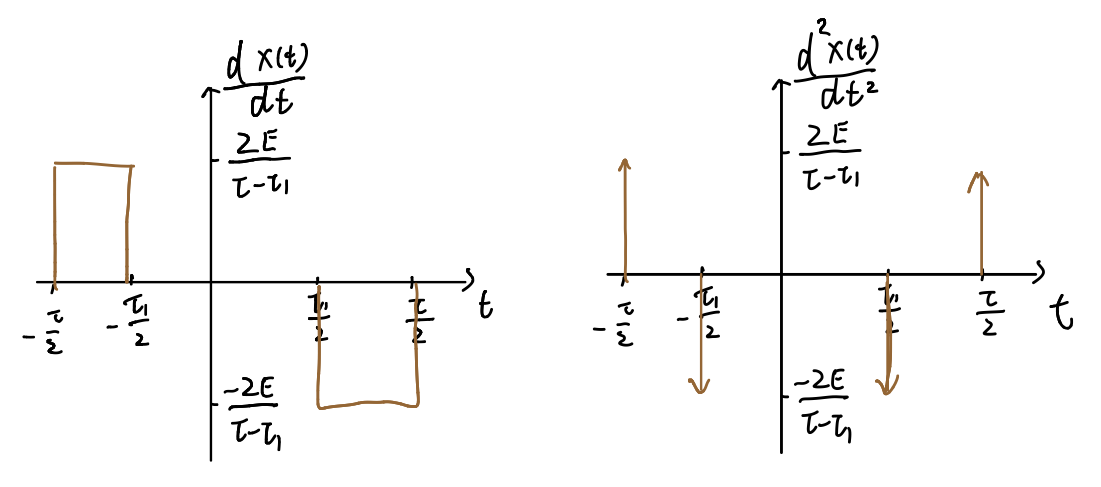
\includegraphics[width=0.6\linewidth]{pics/8-0.png}
	\caption{8-导数}
	\label{fig:13}
\end{figure}
\begin{figure}
	\centering
	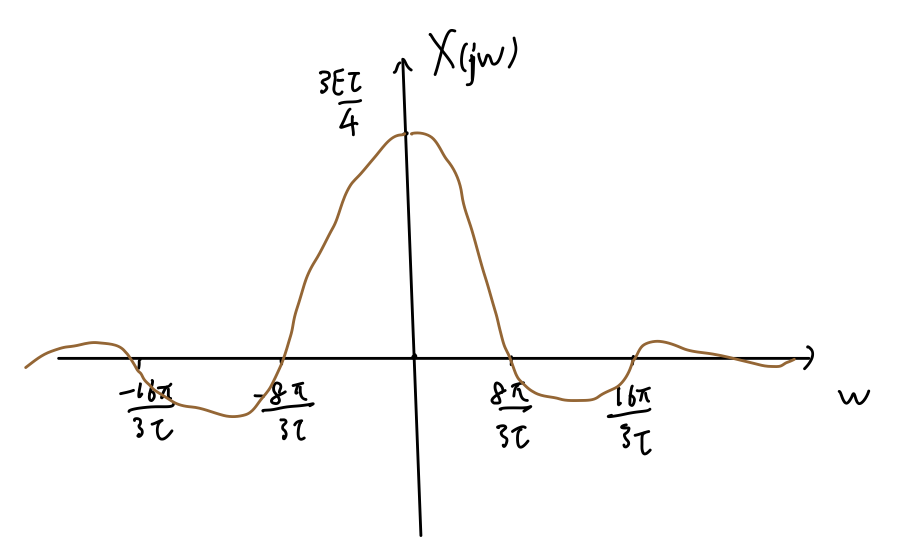
\includegraphics[width=0.6\linewidth]{pics/8-1.png}
	\caption{8-频谱图}
	\label{fig:14}
\end{figure}

\question 若已知$\mathcal{F}[x(t)] = X(j\omega)$,利用傅里叶变换的性质确定下列信号的傅里叶变换。
\begin{enumerate}[(1)]
	\item $tx(2t)$
	\item $(t-2)x(t)$
	\item $(t-2)x(-2t)$
	\item $t\frac{dx(t)}{dt}$
	\item $x(1-t)$
	\item $(1-t)x(1-t)$
	\item $x(2t-5)$
\end{enumerate}


\begin{solution}
	\begin{enumerate}[(1)]
		\item 由频域微分特性得$\mathcal{F}[tx(t)]=j\frac{d}{dw}X(jw)$,再由尺度变换容易得$\mathcal{F}[2tx(2t)]=\frac{j}{2}\frac{d}{d\frac{w}{2}}X(j\frac{w}{2})$,再由线性特性得$\mathcal{F}[tx(2t)]=\frac{j}{2}\frac{d}{dw}X(\frac{jw}{2})$。
		\item $\mathcal{F}[(t-2)x(t)]=\mathcal{F}[(t-2)x(t)]=\mathcal{F}[tx(t)-2x(t)]=\mathcal{F}[tx(t)]-\mathcal{F}[2x(t)]=j\frac{d}{dw}X(jw)-2X(jw)$。
		\item 令$k(t)=x(-2t)$,则有$\mathcal{F}[k(t)]=\frac{1}{2}X(\frac{jw}{-2})$。且$\mathcal{F}[(t-2)k(t)]=j\frac{d}{dw}\frac{X(\frac{jw}{-2})}{2}-X(\frac{jw}{-2})=\frac{j}{2}\frac{d}{dw}X(\frac{jw}{-2})-X(\frac{jw}{-2})$。
		\item 令$k(t)=\frac{d}{dt}x(t)$,则$K(jw)=jwX(jw)$。而$\mathcal{F}[t\frac{d}{dt}x(t)]=\mathcal{F}[tk(t)]=j\frac{d}{dw}K(jw)=-\frac{d}{dw}wX(jw)=-X(jw)-w\frac{d}{dw}X(jw)$。
		\item 因为$\mathcal{F}[x(-t)]=X(-jw)$,所以$\mathcal{F}[x(1-t)]=\mathcal{F}[x(-(t-1))]=X(-jw)e^{-jw}$。
		\item 令$k(t)=x(1-t)$,则有$K(jw)=\mathcal{F}[k(t)]=X(-jw)e^{-jw}$,所以$\mathcal{F}[(1-t)k(t)]=K(jw)-j\frac{d}{dw}K(jw)=X(-jw)e^{-jw}-j[e^{-jw}\frac{d}{dw}X(-jw)-jX(-jw)e^{-jw}]=-je^{-jw}\frac{d}{dw}X(-jw)$。
		\item 因为$\mathcal{F}[x(2t)]=\frac{1}{2}X(\frac{jw}{2})$,所以$\mathcal{F}[2t-5]=\mathcal{F}[x(2(t-\frac{5}{2}))]=\frac{1}{2}X(\frac{jw}{2})e^{-jw\frac{5}{2}}$。
	\end{enumerate}
\end{solution}

\end{questions}

\end{document}